\documentclass[12pt, twoside]{article}
\usepackage[letterpaper, margin=1in, headsep=0.5in]{geometry}
\usepackage[english]{babel}
\usepackage[utf8]{inputenc}
\usepackage{amsmath}
\usepackage{amsfonts}
\usepackage{amssymb}
\usepackage{tikz}
\usepackage{yhmath}
\usetikzlibrary{quotes, angles}

\usepackage{graphicx}
\usepackage{enumitem}
\usepackage{multicol}

\usepackage{fancyhdr}
\pagestyle{fancy}
\fancyhf{}
\renewcommand{\headrulewidth}{0pt} % disable the underline of the header

\fancyhead[RE]{\thepage}
\fancyhead[RO]{\thepage \\ Name: \hspace{3cm}}
\fancyhead[L]{BECA / Dr. Huson / 10th Grade Geometry\\* 6 May 2019}

\begin{document}
\subsubsection*{10.8 Do Now: Volume, density, trig review}
 \begin{enumerate}

   \item $\triangle ABC$ is shown with $m\angle C=90^\circ$ and the lengths of the triangle's sides are $BC=8$, $AC=15$, and $AB=17$.
      \begin{center}
         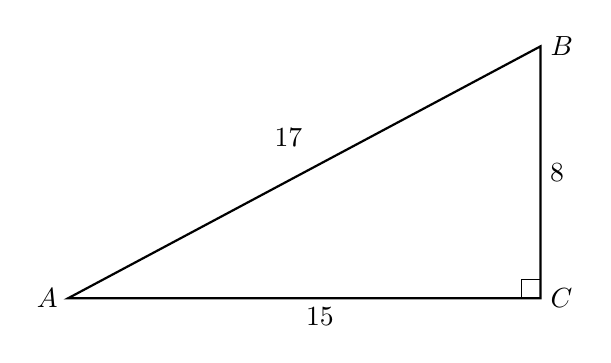
\begin{tikzpicture}[scale=0.4]
           \draw [thick]
           (0,0)node[left]{$A$}--
           (15,0)node[ right]{$C$}--
           (15,8)node[right]{$B$}--cycle;
           \draw (15,0)++(-0.6,0)--++(0,0.6)--+(0.6,0);
           \node at (8,0)[below]{$15$};
           \node at (15,4)[right]{$8$};
           \node at (7,4.5)[above]{$17$};
         \end{tikzpicture}
       \end{center}
        For each item circle True or False.
        \begin{multicols}{2}
         \begin{enumerate}
         \item \quad T \qquad F \qquad $\displaystyle \sin A = \frac{8}{15}$ \vspace{0.25cm}
         \item \quad T \qquad F \qquad $\displaystyle \cos A = \frac{15}{17}$
         \item \quad T \qquad F \qquad $\displaystyle \sin B = \frac{8}{17}$ \vspace{0.25cm}
         \item \quad T \qquad F \qquad $\displaystyle \tan B = \frac{15}{8}$
       \end{enumerate}
     \end{multicols}
  \vspace{1.25cm}

  \item Express each trigonometric ratio to the nearest thousandth and each angle measure to the nearest degree.
    \begin{multicols}{2}
      \begin{enumerate}
        \item $\tan 23^\circ =$ \vspace{0.5cm}
        \item $\cos 79^\circ =$
        \item $\sin^{-1} 0.5 =$ \vspace{0.5cm}
        \item $\cos^{-1} 0.707 =$
      \end{enumerate}
    \end{multicols} \vspace{1.25cm}

  \item In right triangle $ABC$ with $m\angle C=90^\circ$ and $AC \neq BC$. Circle True or False for each statement of trigonometric equivalence.
       \begin{multicols}{2}
        \begin{enumerate}
        \item \quad T \qquad F \qquad $\sin A = \cos B$ \vspace{0.25cm}
        \item \quad T \qquad F \qquad $\tan A = \tan B$
        \item \quad T \qquad F \qquad $\sin B = \cos A$ \vspace{0.25cm}
        \item \quad T \qquad F \qquad $\sin B = \cos B$
      \end{enumerate}
    \end{multicols}

\newpage

   \item Find the area of $\triangle ABC$,  $Area= \frac{1}{2}bh$. The altitude $h$ of the triangle is 11.3 inches and the base $AB=20.7$ in.\\[0.5cm]
   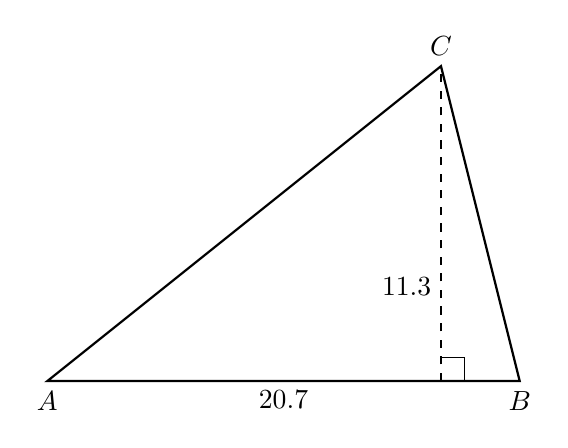
\begin{tikzpicture}[scale=1.0]
     \draw [thick]
       (0,0)node[below]{$A$}--
       (6,0)node[below]{$B$}--
       (5,4)node[above]{$C$} --cycle;
    \draw [dashed] (5,0)--(5,4);
    \draw (5,0)++(0.3,0)--++(0,0.3)--+(-0.3,0);
    \node at (5,1.2)[left]{$11.3$};
    \node at (3,0)[below]{$20.7$};
  \end{tikzpicture} \vspace{3.0cm}

  \item On the set of axes below, $\triangle ABC$, altitude $\overline{GC}$, and  median $\overline{MC}$ are drawn.
    \begin{center}
      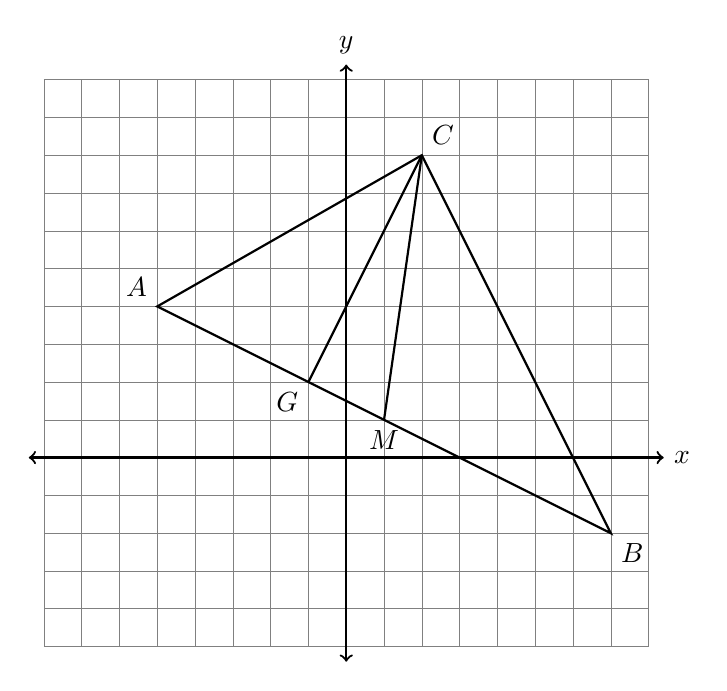
\begin{tikzpicture}[scale=.48]
        \draw [help lines] (-8,-5) grid (8,10);
        \draw [thick, <->] (-8.4,0) -- (8.4,0) node [right] {$x$};
        \draw [thick, <->] (0,-5.4)--(0,10.4) node [above] {$y$};
        \draw [thick]
          (-5,4) node[above left] {$A$}--
          (7,-2) node[below right] {$B$}--
          (2,8) node[above right] {$C$}--
          cycle;
        \draw [thick] (1,1) node[below] {$M$}--(2,8);
        \draw [thick] (-1,2) node[below left] {$G$}--(2,8);
      \end{tikzpicture}
    \end{center}
      Determine which equations represent the area of the triangle, circling True or False.
      \begin{multicols}{2}
       \begin{enumerate}
       \item \quad T \quad F \quad $\displaystyle Area_\triangle = \frac{(AC)(AB)}{2}$ \vspace{0.25cm}
       \item \quad T \quad F \quad $\displaystyle Area_\triangle = \frac{(CG)(BC)}{2}$
       \item \quad T \quad F \quad $\displaystyle Area_\triangle = \frac{(CM)(AB)}{2}$ \vspace{0.25cm}
       \item \quad T \quad F \quad $\displaystyle Area_\triangle = \frac{(CG)(AB)}{2}$
      \end{enumerate}
      \end{multicols}
      \vspace{0.25cm}

  \end{enumerate}
  \newpage
  \setcounter{page}{1}
\subsubsection*{10.8 Classwork: Compound volumes \& angle of elevation}
 \begin{enumerate}

  \item A vendor is using an 8-ft by 8-ft tent for a craft fair. The legs of the tent are 9 ft tall and the top forms a square pyramid with a height of 3 ft.\\[1cm]
    \includegraphics[width=0.4\textwidth]{tent_Jan2019-9.png}\\[0.5cm]
    What is the volume, in cubic feet, of space the tent occupies? \vspace{3cm}

  \item A walking path at a local park is modeled on the grid below, where the length of each grid square is 10 feet. The town needs to submit paperwork to pave the walking path. Determine and state, to the \emph{nearest square foot}, the area of the walking path.\\[0.3cm]
    \includegraphics[width=0.6\textwidth]{path_Jan2019-31.png} \vspace{3cm}

  \item Lawrence has a rectangular pool 22 ft long, 15 ft wide, and 5 ft deep.
    \begin{enumerate}
      \item Find the volume of the pool in cubic feet. \vspace{2cm}
      \item Find the volume of the pool in gallons, where $1 \mathrm{ ft}^3$ water $= 1.48$ gallons. \vspace{2cm}
      \item If Lawrence filled his pool using city water at a rate of \$3.95 per 100 gallons of water, find the total cost.
    \end{enumerate} \vspace{2cm}

\item As modeled in the diagram below, an access ramp that is 20 feet long has an angle of elevation of $5^\circ$. Determine and state the vertical height of the ramp, to the \emph{nearest tenth of a foot}.\\[0.3cm]
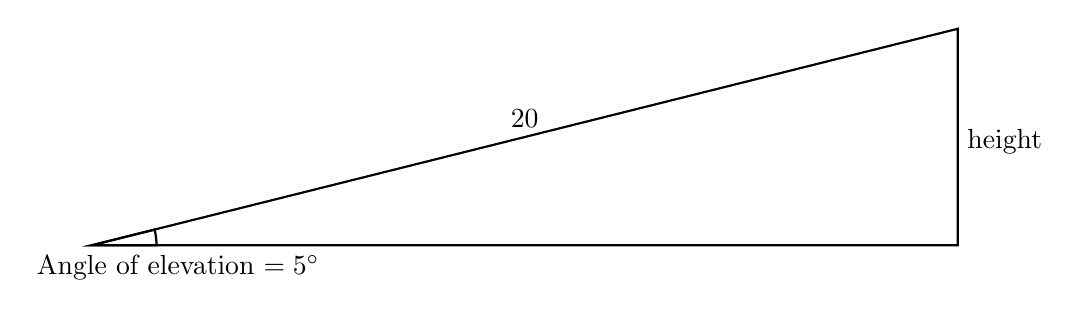
\begin{tikzpicture}[scale=1.1]
  \draw [thick] (10,0)--(0,0)--(10,2.5)--cycle;
  \draw [thick] (0,0)--(0.75,0) arc [start angle=0, end angle=14, radius=0.75]--cycle;
  \node at (1,0)[below]{Angle of elevation $=5^\circ$};
  \node at (10,1.2)[right]{height};
  \node at (5,1.25)[above]{20};
\end{tikzpicture} \vspace{3cm}

\item Yolanda is making a springboard to use for gymnastics. She has 8-inch-tall springs and wants to form a $16.5^\circ$ angle with the base, as modeled in the diagram below.\\[0.3cm]
  \includegraphics[width=0.4\textwidth]{spring_Aug2018-6.png}\\
To the \emph{nearest tenth of a inch}, what will be the length of the springboard, $x$?
  \vspace{0.5cm}


  \item From a point on the ground one-half mile from the base of a historic monument, the angle of elevation to its top is $11.87^\circ$. To the nearest foot, what is the height of the monument?\\[1cm]
    \begin{tikzpicture}[scale=1.1]
      \draw [dashed] (10,0)--(0,0)--(10,2);
      \draw [thick, ->] (10,0)--(10,2);
      \draw (10,0)++(-0.3,0)--++(0,0.3)--+(0.3,0);
      \fill [gray] (0,0)--(0.75,0) arc [start angle=0, end angle=11.3, radius=0.75]--cycle;
      \node at (1,0)[below]{$11.87^\circ$};
      \node at (10,1)[right]{Monument};
      \node at (6,0)[below]{One-half mile};
    \end{tikzpicture} \vspace{3cm}

\newpage
  \item How many cubic inches are in the volume of a cube one foot on each side?

  \item A child’s tent can be modeled as a pyramid with a square base whose sides measure 60 inches and whose height measures 84 inches. What is the volume of the tent, to the \emph{nearest cubic foot}?

  \item Find the volume of a cylinder with radius $r=3$ and height $h=10$. Leave your answer in terms of $\pi$ (not a decimal). \vspace{2.5cm}

  \item Find the weight of $60$ liters of gasoline, given that the density of gasoline is $0.73$ kilograms per liter. \vspace{3.0cm}

  \item A circle with a diameter of 10 cm and a central angle of $30^\circ$ is drawn below.
       \begin{center}
       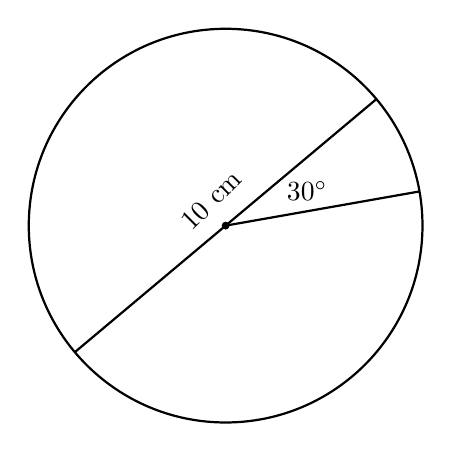
\begin{tikzpicture}[scale=.5]
         \draw [thick] (0,0) circle[radius=5];
         \draw [thick] (40:5)--(220:5);
         \draw [thick] (0,0)--(10:5);
         \fill (0,0) circle[radius=0.1];
         \draw (23:2.25) node{$30^\circ$};
         \draw (120:0.75) node[rotate=45]{$10$ cm};
         %\draw (75:1.8) node[above] {$C$};
         %\draw (290:5) node[below] {$D$};
       \end{tikzpicture}
     \end{center}
  What is the area, to the \emph{nearest tenth of a square centimeter}, of the sector formed by the $30^\circ$ angle?

\end{enumerate}
\end{document}

\item Theresa has a rectangular pool 30 ft long, 15 ft wide, and 4 ft deep. Theresa fills her pool using city water at a rate of \$3.95 per 100 gallons of water.\\
Nancy has a circular pool with a diameter of 24 ft and a depth of 4 ft. Nancy fills her pool with a water delivery service at a rate of \$200 per 6000 gallons.\\
If Theresa and Nancy both fill their pools 6 inches from the top of the pool, determine and state who paid more to fill her pool. ($1 \mathrm{ft}^3$ water $= 1.48$ gallons)

\item As modeled in the diagram below, an access ramp starts on flat ground and ends at the beginning of the top step. Each step is 6 inches tall and 8 inches deep. \\[0.3cm]
  \includegraphics[width=0.8\textwidth]{ramp_Jan2019-34.png}\\
If the angle of elevation of the ramp is $4.76^\circ$, determine and state the length of the ramp, to the \emph{nearest tenth of a foot}.\\[2cm]
Determine and state, to the \emph{nearest tenth of a foot}, the horizontal distance, $d$, from the bottom of the stairs to the bottom of the ramp.
